\section{Mức độ 5,6 điểm}
\Opensolutionfile{ans}[ans/CD6/Muc_5_6]
\setcounter{dang}{0}
\setcounter{ex}{0}
\begin{dang}{Bài toán tương giao đồ thị thông qua đồ thị, bảng biến thiên}
\end{dang}
\begin{ex}[Đề Minh Họa 2020 - Lần 1] %[2D1Y5-4]
Cho hàm số $f(x)$ có bảng biến thiên như sau
\begin{center}

\begin{tikzpicture}
\tkzTabInit[nocadre=true,lgt=1.2,espcl=2.5,deltacl=0.6]
{$x$ /0.6, $f'(x)$ /0.6, $f(x)$ /2.5}
{$-\infty$,$2$,$3$,$+\infty$}
\tkzTabLine{,+,$0$,-,$0$,+,}
\tkzTabVar{-/$-\infty$,+/$1$,-/$0$,+/$+\infty$}
\end{tikzpicture}
\end{center}
Số nghiệm của phương trình $3f(x)-2=0$ là
\choice
{$2$}
{$0$}
{\True $3$}
{$1$}
\loigiai{
Ta có $3f(x)-2=0\Leftrightarrow f(x)=\dfrac{2}{3}$.
\begin{center}
\begin{tikzpicture}
\tkzTabInit[nocadre=true,lgt=1.2,espcl=2.5,deltacl=0.6]
{$x$ /0.6, $f'(x)$ /0.6, $f(x)$ /2.5}
{$-\infty$,$2$,$3$,$+\infty$}
\tkzTabLine{,+,$0$,-,$0$,+,}
\tkzTabVar{-/$-\infty$,+/$1$,-/$0$,+/$+\infty$}
\draw (1.3,-2.5)--(9.5,-2.5)node[below left]{$y=\dfrac{2}{3}$};
\end{tikzpicture}
\end{center}
Căn cứ vào bảng biến thiên thì phương trinh $3f(x)-2=0\Leftrightarrow f(x)=\dfrac{2}{3}$ có $3$ nghiệm phân biệt.}
\end{ex}

%%% CÂU 2
\begin{ex}[Mã 101 - 2020 Lần 1] %[2D1Y5-4]
\immini{
Cho hàm số bậc ba $y=f(x)$ có đồ thị là đường cong trong hình bên. Số nghiệm thực của phương trình $f(x)=-1$ là
\choice
{\True $3$}
{$1$}
{$0$}
{$2$}
}{
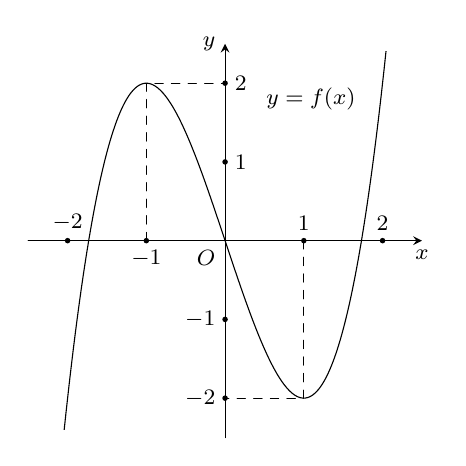
\begin{tikzpicture}[scale=1, font=\footnotesize, line join=round, line cap=round,>=stealth]
\def\a{1} \def\b{0} \def\c{-3} \def\d{0}
\def\xmin{-2.5} \def\xmax{2.5}
\def\ymin{-2.5} \def\ymax{2.5}
\draw[->] (\xmin,0)--(\xmax,0) node [below]{$x$};
\draw[->] (0,\ymin)--(0,\ymax) node [left]{$y$};
\node at (0,0) [below left]{$O$};
\clip (\xmin+0.1,\ymin+0.1) rectangle (\xmax-0.1,\ymax-0.1);
\draw[smooth,samples=300] plot(\x,{\a*(\x)^3+\b*(\x)^2+\c*(\x)+\d});
\draw[dashed] (-1,0)node[below]{$-1$}--(-1,2)--(0,2)node[right]{$2$}
(1,0)node[above]{$1$}--(1,-2)--(0,-2)node[left]{$-2$};
\fill (-1,0) circle (1.0pt) (1,0) circle (1.0pt) (0,2) circle (1.0pt)
(0,-2) circle (1.0pt) (-2,0) circle (1.0pt) node[above]{$-2$}
(0,-1) circle (1.0pt) node[left]{$-1$}
(2,0) circle (1.0pt) node[above]{$2$}
(0,1) circle (1.0pt) node[right]{$1$};
\node at (0.4,1.8)[right]{$y=f(x)$};
\end{tikzpicture}
}
\loigiai{
Số nghiệm thực của phương trình $f(x)=-1$ chính là số giao điểm của đồ thị hàm số $y=f(x)$ và đường thẳng $y=-1$.
\begin{center}
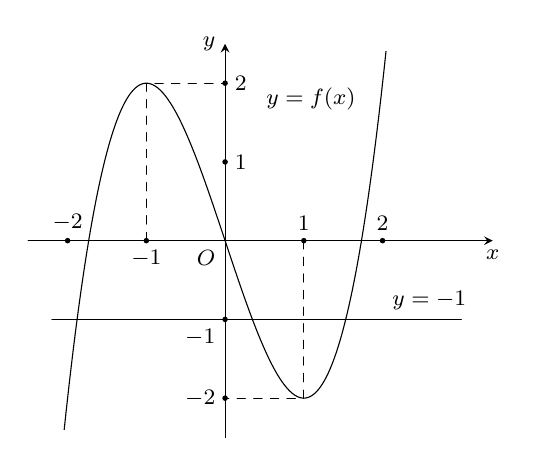
\begin{tikzpicture}[scale=1, font=\footnotesize, line join=round, line cap=round,>=stealth]
\def\a{1} \def\b{0} \def\c{-3} \def\d{0}
\def\xmin{-2.5} \def\xmax{3.4}
\def\ymin{-2.5} \def\ymax{2.5}
\draw[->] (\xmin,0)--(\xmax,0) node [below]{$x$};
\draw[->] (0,\ymin)--(0,\ymax) node [left]{$y$};
\node at (0,0) [below left]{$O$};
\clip (\xmin+0.1,\ymin+0.1) rectangle (\xmax-0.1,\ymax-0.1);
\draw[smooth,samples=300] plot(\x,{\a*(\x)^3+\b*(\x)^2+\c*(\x)+\d});
\draw[dashed] (-1,0)node[below]{$-1$}--(-1,2)--(0,2)node[right]{$2$}
(1,0)node[above]{$1$}--(1,-2)--(0,-2)node[left]{$-2$};
\fill (-1,0) circle (1.0pt) (1,0) circle (1.0pt) (0,2) circle (1.0pt)
(0,-2) circle (1.0pt) (-2,0) circle (1.0pt) node[above]{$-2$}
(0,-1) circle (1.0pt) node[below left]{$-1$}
(2,0) circle (1.0pt) node[above]{$2$}
(0,1) circle (1.0pt) node[right]{$1$};
\node at (0.4,1.8)[right]{$y=f(x)$};
\draw (-2.2,-1)--(3,-1);
\node at (2,-1)[above right]{$y=-1$};
\end{tikzpicture}
\end{center}
Từ hình vẽ suy ra $3$ nghiệm.}
\end{ex}

%%% CÂU 3
\begin{ex}[Mã 102 - 2020 Lần 1] %[2D1Y5-4]
Cho hàm số bậc ba $y=f(x)$ có đồ thị là đường cong trong hình bên. Số nghiệm thực của phương trình $f(x)=1$ là
\begin{center}
\begin{tikzpicture}[scale=1, font=\footnotesize, line join=round, line cap=round,>=stealth]
\def\a{-1} \def\b{0} \def\c{3} \def\d{1}
\def\xmin{-2.3} \def\xmax{3}
\def\ymin{-1.5} \def\ymax{4}
\draw[->] (\xmin,0)--(\xmax,0) node [below]{$x$};
\draw[->] (0,\ymin)--(0,\ymax) node [left]{$y$};
\node at (0,0) [below left]{$O$};
\clip (\xmin+0.1,\ymin+0.1) rectangle (\xmax-0.1,\ymax-0.1);
\draw[smooth,samples=300] plot(\x,{\a*(\x)^3+\b*(\x)^2+\c*(\x)+\d});
\draw[dashed] (-1,0)node[above]{$-1$}--(-1,-1)--(0,-1)node[right]{$-1$}
(1,0)node[below]{$1$}--(1,3)--(0,3)node[left]{$3$};
\end{tikzpicture}
\end{center}
\choice
{$0$}
{\True $3$}
{$1$}
{$2$}
\loigiai{
Ta thấy đường thẳng $y=1$ cắt đồ thị hàm số $y=f(x)$ tại $3$ điểm phân biệt nên phương trình $f(x)=1$ có $3$ nghiệm phân biệt.}
\end{ex}

%%% CÂU 4
\begin{ex}[Mã 103 - 2020 Lần 1] %[2D1Y5-4]
\immini{
Cho hàm số bậc ba $y=f(x)$ có đồ thị là đường cong trong hình bên. Số nghiệm thực của phương trình $f(x)=1$ là
\choice
{$1$}
{$0$}
{$2$}
{\True $3$}
}{
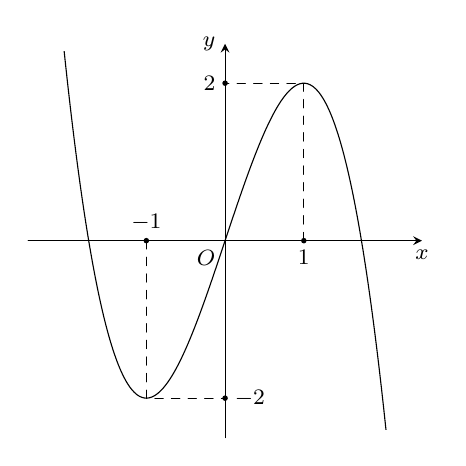
\begin{tikzpicture}[scale=1, font=\footnotesize, line join=round, line cap=round,>=stealth]
\def\a{-1} \def\b{0} \def\c{3} \def\d{0}
\def\xmin{-2.5} \def\xmax{2.5}
\def\ymin{-2.5} \def\ymax{2.5}
\draw[->] (\xmin,0)--(\xmax,0) node [below]{$x$};
\draw[->] (0,\ymin)--(0,\ymax) node [left]{$y$};
\node at (0,0) [below left]{$O$};
\clip (\xmin+0.1,\ymin+0.1) rectangle (\xmax-0.1,\ymax-0.1);
\draw[smooth,samples=300] plot(\x,{\a*(\x)^3+\b*(\x)^2+\c*(\x)+\d});
\draw[dashed] (-1,0)node[above]{$-1$}--(-1,-2)--(0,-2)node[right]{$-2$}
(1,0)node[below]{$1$}--(1,2)--(0,2)node[left]{$2$};
\fill (-1,0) circle (1.0pt) (0,-2) circle (1.0pt)
(1,0) circle (1.0pt) (0,2) circle (1.0pt) ;
\end{tikzpicture}
}
\loigiai{
Từ đồ thị hàm số ta có số nghiệm thực của phương trình $f(x)=1$ là $3$.}
\end{ex}

%%% CÂU 5
\begin{ex}[Mã 104 - 2020 Lần 1] %[2D1Y5-4]
Cho hàm số bậc ba $y=f(x)$ có đồ thị là đường cong trong hình vẽ.
\begin{center}
\begin{tikzpicture}[scale=1, font=\footnotesize, line join=round, line cap=round,>=stealth]
\def\a{1} \def\b{0} \def\c{-3} \def\d{1}
\def\xmin{-2.3} \def\xmax{3}
\def\ymin{-1.5} \def\ymax{4}
\draw[->] (\xmin,0)--(\xmax,0) node [below]{$x$};
\draw[->] (0,\ymin)--(0,\ymax) node [left]{$y$};
\node at (0,0) [below left]{$O$};
\clip (\xmin+0.1,\ymin+0.1) rectangle (\xmax-0.1,\ymax-0.1);
\draw[smooth,samples=300] plot(\x,{\a*(\x)^3+\b*(\x)^2+\c*(\x)+\d});
\draw[dashed] (-1,0)node[below]{$-1$}--(-1,3)--(0,3)node[right]{$3$}
(1,0)node[above]{$1$}--(1,-1)--(0,-1)node[left]{$-1$};
\end{tikzpicture}
\end{center}
Số nghiệm thực của phương trình $f(x)=2$ là
\choice
{$0$}
{\True $3$}
{$1$}
{$2$}
\loigiai{
Ta có số nghiệm của phương trình là số giao điểm của đồ thị hàm số $y=f(x)$ với đường thẳng $y=2$.\\
Dựa vào đồ thị ta có phương trình có ba nghiệm phân biệt.}
\end{ex}

%%% CÂU 6
\begin{ex}[Mã 101 - 2019] %[2D1Y5-4]
Cho hàm số $f(x)$ có bảng biến thiên như sau:
\begin{center}

\begin{tikzpicture}
\tkzTabInit[nocadre=true,lgt=1.2,espcl=2.5,deltacl=0.6]
{$x$ /0.6,$f'(x)$ /0.6,$f(x)$ /2}
{$-\infty$,$-2$,$0$,$2$,$+\infty$}
\tkzTabLine{,+,$0$,-,$0$,+,$0$,-,}
\tkzTabVar{-/$-\infty$, +/$3$,-/$-1$,+/$3$,-/$-\infty$}
\end{tikzpicture}
\end{center}
Số nghiệm thực của phương trình $2f(x)-3=0$ là
\choice
{$2$}
{$1$}
{\True $4$}
{$3$}
\loigiai{
Ta có $2f(x)-3=0\Leftrightarrow f(x)=\dfrac{3}{2}$.\\
Số nghiệm của phương trình bằng số giao điểm của đồ thị hàm số $y=f(x)$ và đường thẳng $y=\dfrac{3}{2}$.\\
Dựa vào bảng biến thiên của $f(x)$ ta có số giao điểm của đồ thị hàm số $y=f(x)$ và đường thẳng $y=\dfrac{3}{2}$ là $4$.}
\end{ex}

%%% CÂU 7
\begin{ex}[Mã 101 - 2018] %[2D1Y5-4]
Cho hàm số $f(x)=ax^3+bx^2+cx+d,(a,b,c,d\in\mathbb{R})$. Đồ thị của hàm số $y=f(x)$ như hình vẽ. Số nghiệm thực của phương trình $3f(x)+4=0$ là
\begin{center}
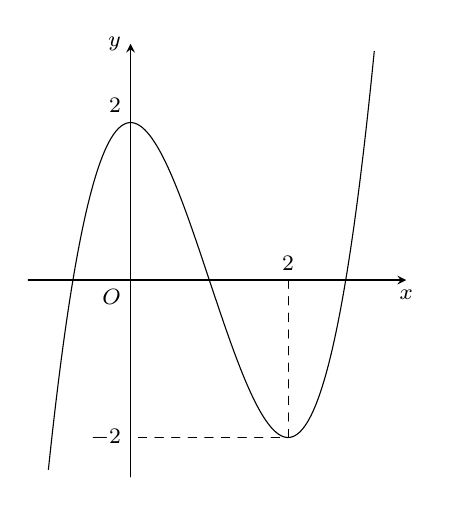
\begin{tikzpicture}[scale=1, font=\footnotesize, line join=round, line cap=round,>=stealth]
\def\a{1} \def\b{-3} \def\c{0} \def\d{2}
\def\xmin{-1.3} \def\xmax{3.5}
\def\ymin{-2.5} \def\ymax{3}
\draw[->] (\xmin,0)--(\xmax,0) node [below]{$x$};
\draw[->] (0,\ymin)--(0,\ymax) node [left]{$y$};
\node at (0,0) [below left]{$O$};
\clip (\xmin+0.1,\ymin+0.1) rectangle (\xmax-0.1,\ymax-0.1);
\draw[smooth,samples=300] plot(\x,{\a*(\x)^3+\b*(\x)^2+\c*(\x)+\d});
\draw[dashed] (2,0)node[above]{$2$}--(2,-2)--(0,-2)node[left]{$-2$};
\node at (0,2)[above left]{$2$};
\end{tikzpicture}
\end{center}
\choice
{$2$}
{$0$}
{$1$}
{\True $3$}
\loigiai{
Ta có $3f(x)+4=0\Leftrightarrow f(x)=-\dfrac{4}{3}\quad(*)$\\
$(*)$ là phương trình hoành độ giao điểm của đồ thị hàm số $y=f(x)$ và đường thẳng $y=-\dfrac{4}{3}$.\\
Dựa vào đồ thị hàm số, ta thấy $(*)$ có $3$ nghiệm.}
\end{ex}

%%% CÂU 8
\begin{ex}[Mã 102 - 2018] %[2D1Y5-4]
Cho hàm số $f(x)=ax^4+bx^2+c,(a,b,c\in \mathbb{R})$. Đồ thị của hàm số $y=f(x)$ như hình vẽ bên.
\begin{center}
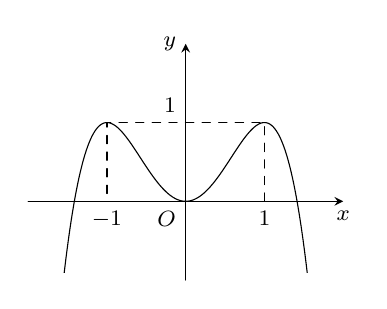
\begin{tikzpicture}[scale=1, font=\footnotesize, line join=round, line cap=round,>=stealth]
\def\a{-1} \def\b{2} \def\c{0}
\def\xmin{-2} \def\xmax{2}
\def\ymin{-1} \def\ymax{2}
\draw[->] (\xmin,0)--(\xmax,0) node [below]{$x$};
\draw[->] (0,\ymin)--(0,\ymax) node [left]{$y$};
\node at (0,0) [below left]{$O$};
\clip (\xmin+0.1,\ymin+0.1) rectangle (\xmax-0.1,\ymax-0.1);
\draw[smooth,samples=300,domain=-1.8:1.8] plot(\x,{\a*(\x)^4+\b*(\x)^2+\c});
\draw[dashed] (1,0)node[below]{$1$}--(1,1)--(-1,1)--(-1,0)node[below]{$-1$};
\node at (0,1)[above left]{$1$};
\end{tikzpicture}
\end{center}
Số nghiệm của phương trình $4f(x)-3=0$ là
\choice
{$2$}
{$0$}
{\True $4$}
{$3$}
\loigiai{
Ta có $4f(x)-3=0\Leftrightarrow f(x)=\dfrac{3}{4}$.
\begin{center}
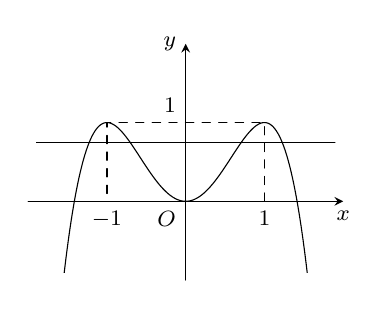
\begin{tikzpicture}[scale=1, font=\footnotesize, line join=round, line cap=round,>=stealth]
\def\a{-1} \def\b{2} \def\c{0}
\def\xmin{-2} \def\xmax{2}
\def\ymin{-1} \def\ymax{2}
\draw[->] (\xmin,0)--(\xmax,0) node [below]{$x$};
\draw[->] (0,\ymin)--(0,\ymax) node [left]{$y$};
\node at (0,0) [below left]{$O$};
\clip (\xmin+0.1,\ymin+0.1) rectangle (\xmax-0.1,\ymax-0.1);
\draw[smooth,samples=300,domain=-1.8:1.8] plot(\x,{\a*(\x)^4+\b*(\x)^2+\c});
\draw[dashed] (1,0)node[below]{$1$}--(1,1)--(-1,1)--(-1,0)node[below]{$-1$};
\node at (0,1)[above left]{$1$};
\draw (-2,0.75)--( 2,0.75);
\end{tikzpicture}
\end{center}
Đường thẳng $y==\dfrac{3}{4}$ cắt đồ thị hàm số $y=f(x)$ tại $4$ điểm phân biệt nên phương trình đã cho có $4$ nghiệm phân biệt.}
\end{ex}

%%% CÂU 9
\begin{ex}[Mã 103 - 2019] %[2D1Y5-4]
Cho hàm số $f(x)$ bảng biến thiên như sau:
\begin{center}

\begin{tikzpicture}
\tkzTabInit[nocadre=true,lgt=1.2,espcl=2.5,deltacl=0.6]
{$x$ /0.6, $y'$ /0.6, $y$ /2.5}
{$-\infty$,$-1$,$2$,$+\infty$}
\tkzTabLine{,-,$0$,+,$0$,-,}
\tkzTabVar{+/$+\infty$,-/$-1$,+/$2$,-/$-\infty$}
\end{tikzpicture}
\end{center}
Số nghiệm thực của phương trình $2f(x)-3=0$ là
\choice
{\True $3$}
{$0$}
{$1$}
{$2$}
\loigiai{
Ta có $2f(x)-3=0\Leftrightarrow f(x)=\dfrac{3}{2}.\quad(1)$\\
Số nghiệm thực của phương trình $(1)$ bằng số giao điểm của đồ thị hàm số $y=f(x)$ với đường thẳng $y=\dfrac{3}{2}$.\\
Từ bảng biến thiên đã cho của hàm số $f(x)$, ta thấy đường thẳng $y=\dfrac{3}{2}$ cắt đồ thị hàm số $y=f(x)$ tại ba điểm phân biệt.\\
Do đó phương trình $(1)$ có ba nghiệm thực phân biệt.}
\end{ex}

%%% CÂU 10
\begin{ex}[Mã 103 - 2018] %[2D1Y5-4]
Cho hàm số $f(x)$ liên tục trên $[-2;2]$ và có đồ thị như hình vẽ bên. Số nghiệm thực của phương trình $3f(x)-4=0$ trên đoạn $[-2;2]$ là
\begin{center}
\begin{tikzpicture}[scale=1, font=\footnotesize, line join=round, line cap=round,>=stealth]
\def\a{1} \def\b{0} \def\c{-3} \def\d{1}
\def\xmin{-2.8} \def\xmax{3}
\def\ymin{-1.8} \def\ymax{4}
\draw[->] (\xmin,0)--(\xmax,0) node [below]{$x$};
\draw[->] (0,\ymin)--(0,\ymax) node [left]{$y$};
\node at (0,0) [below left]{$O$};
\clip (\xmin+0.1,\ymin+0.1) rectangle (\xmax-0.1,\ymax-0.1);
\draw[smooth,samples=300] plot(\x,{\a*(\x)^3+\b*(\x)^2+\c*(\x)+\d});
\draw[dashed] (-1,0)node[below]{$-1$}--(-1,3)--(2,3)--(2,0)node[below]{$2$}
(1,0)node[above]{$1$}--(1,-1)--(-2,-1)--(-2,0)node[above left]{$-2$};
\node at (0,-1)[below left]{$-1$};
\node at (0,3)[above right]{$3$};
\end{tikzpicture}
\end{center}
\choice
{$4$}
{\True $3$}
{$1$}
{$2$}
\loigiai{
Ta có $3f(x)-4=0\Leftrightarrow f(x)=\dfrac{4}{3}$.\\
Dựa vào đồ thị, ta thấy đường thẳng $y=\dfrac{4}{3}$ cắt $y=f(x)$ tại $3$ điểm phân biệt nên phương trình đã cho có $3$ nghiệm phân biệt.}
\end{ex}

%%% CÂU 11
\begin{ex}[Mã 102 - 2019] %[2D1Y5-4]
Cho hàm số $f(x)$ có bảng biến thiên như sau
\begin{center}

\begin{tikzpicture}
\tkzTabInit[nocadre=true,lgt=1.2,espcl=2.5,deltacl=0.6]
{$x$ /0.6,$f'(x)$ /0.6,$f(x)$ /2}
{$-\infty$,$-2$,$0$,$2$,$+\infty$}
\tkzTabLine{,-,$0$,+,$0$,-,$0$,+,}
\tkzTabVar{+/$+\infty$, -/$-1$,+/$2$,-/$-1$,+/$+\infty$}
\end{tikzpicture}
\end{center}
Số nghiệm thực của phương trình $3f(x)-5=0$ là
\choice
{$3$}
{\True $4$}
{$0$}
{$2$}
\loigiai{
Bảng biến thiên
\begin{center}
\begin{tikzpicture}
\tkzTabInit[nocadre=true,lgt=1.2,espcl=2.5,deltacl=0.6]
{$x$ /0.6,$f'(x)$ /0.6,$f(x)$ /2}
{$-\infty$,$-2$,$0$,$2$,$+\infty$}
\tkzTabLine{,-,$0$,+,$0$,-,$0$,+,}
\tkzTabVar{+/$+\infty$, -/$-1$,+/$2$,-/$-1$,+/$+\infty$}
\draw (1.4,-2.3)--(11,-2.3)node[right]{$y=\dfrac{5}{3}$};
\end{tikzpicture}
\end{center}
Xét phương trình $3f(x)-5=0\Leftrightarrow f(x)=\dfrac{5}{3}$.\\
Số nghiệm của phương trình bằng số giao điểm của đồ thị hàm số $(C)\colon y=f(x)$ và đường thẳng $d\colon y=\dfrac{5}{3}$.\\
Dựa vào bảng biến thiên ta thấy đường thẳng $d$ cắt đồ thị $(C)$ tại bốn điểm phân biệt.}
\end{ex}

%%% CÂU 12
\begin{ex}[THCS - THPT Nguyễn Khuyến 2019] %[2D1B5-4]
Cho hàm số $y=f(x)$ liên tục trên $\mathbb{R}$ và có đồ thị như hình vẽ.
\begin{center}
\begin{tikzpicture}[scale=0.7, font=\footnotesize, line join=round, line cap=round,>=stealth]
\draw[->] (-1,0)--(7,0) node[below]{$x$};
\draw[->] (0,-4)--(0,2) node[right]{$y$};
\node at (0,0) [below left]{$O$};
\path
(-0.09,-3.23) coordinate (A)
(2,1) coordinate (B)
(4,-3) coordinate (C)
(6.3,1.8) coordinate (D)
;
\draw
(A) .. controls +(85:0.4) and +(-170:0.6) ..
(B) .. controls +(-10:0.6) and +(180:0.4) ..
(C) .. controls +(10:0.6) and +(-100:.5) ..(D);
\draw[dashed] (0,1)node[left]{$1$}--(2,1)--(2,0)
(0,-3)node[left]{$-3$}--(4,-3)--(4,0);
\end{tikzpicture}
\end{center}
Số nghiệm của phương trình $\left|f(x)\right|=2$ là
\choice
{$3$}
{$2$}
{\True $4$}
{$6$}
\loigiai{
*Đồ thị $y=\left|f(x)\right|$\\
- Bước 1: Giữ nguyên phần đồ thị của $y=f(x)$ nằm phía trên $Ox$.\\
- Bước 2: Lấy đối xứng phần đồ thị của $y=f(x)$ nằm phía dưới $Ox$ qua trục hoành.\\
- Bước 3: Xóa phần đồ thị của $y=f(x)$ nằm phía dưới trục hoành
\begin{center}
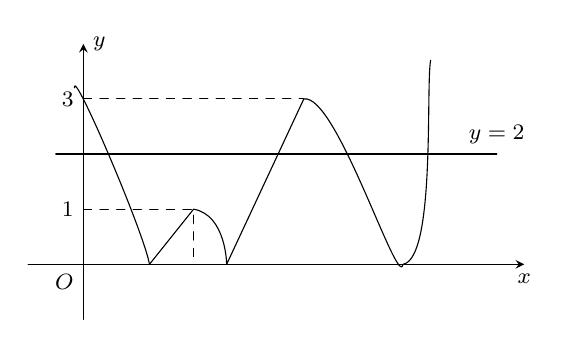
\begin{tikzpicture}[scale=0.7, font=\footnotesize, line join=round, line cap=round,>=stealth]
\draw[->] (-1,0)--(8,0) node[below]{$x$};
\draw[->] (0,-1)--(0,4) node[right]{$y$};
\node at (0,0) [below left]{$O$};
\path
(-0.16,3.2) coordinate (A)
(1.2,0) coordinate (A1)
(2,1) coordinate (B)
(2.6,0) coordinate (B1)
(4,3) coordinate (C)
(5.8,0) coordinate (C1)
(6.3,3.7) coordinate (D)
;
\draw
(A) .. controls +(95:0.4) and +(100:0.6) ..
(A1) .. controls +(170:0) and +(85:0) ..
(B) .. controls +(-10:0.6) and +(120:0) ..
(B1) .. controls +(120:0) and +(85:0) ..
(C) .. controls +(10:0.6) and +(-100:.5) ..
(C1) .. controls +(10:0.6) and +(-100:.5) ..(D);
\draw[dashed] (0,1)node[left]{$1$}--(2,1)--(2,0)
(0,3)node[left]{$3$}--(4,3);
\draw (-0.5,2)--(7.5,2)node[above]{$y=2$};
\end{tikzpicture}
\end{center}
Số nghiệm của phương trình $\left|f(x)\right|=2$ cũng chính là số giao điểm cũng đồ thị hàm số $y=\left|f(x)\right|$ và đường thẳng $y=2$. Dựa vào hình vẽ trên, ta thấy có $4$ giao điểm.\\
*Cách giải khác:
$\left|f(x)\right|=2\Leftrightarrow \hoac{& f(x)=2 \\ &  f(x)=-2}$, dựa vào đồ thị suy ra phương trình đã cho có $4$ nghiệm.}
\end{ex}

%%% CÂU 13
\begin{ex}[Mã 104 - 2019] %[2D1Y5-4]
Cho hàm số $f(x)$ có bảng biến thiên như sau
\begin{center}

\begin{tikzpicture}
\tkzTabInit[nocadre=true,lgt=1.2,espcl=2.5,deltacl=0.6]
{$x$ /0.6, $f'(x)$ /0.6, $f(x)$ /2.5}
{$-\infty$,$-1$,$2$,$+\infty$}
\tkzTabLine{,+,$0$,-,$0$,+,}
\tkzTabVar{-/$-\infty$,+/$2$,-/$-2$,+/$+\infty$}
\end{tikzpicture}
\end{center}
Số nghiệm thực của phương trình $2f(x)+3=0$ là
\choice
{$0$}
{$1$}
{$2$}
{\True $3$}
\loigiai{
\begin{center}
\begin{tikzpicture}
\tkzTabInit[nocadre=true,lgt=1.2,espcl=2.5,deltacl=0.6]
{$x$ /0.6, $f'(x)$ /0.6, $f(x)$ /2.5}
{$-\infty$,$-1$,$2$,$+\infty$}
\tkzTabLine{,+,$0$,-,$0$,+,}
\tkzTabVar{-/$-\infty$,+/$2$,-/$-2$,+/$+\infty$}
\draw (1.4,-2.3)--(9.3,-2.3)node[below left]{$y=-\dfrac{3}{2}$};
\end{tikzpicture}
\end{center}
Ta có $2 f(x)+3=0\Leftrightarrow f(x)=-\dfrac{3}{2}$.\\
Dựa vào bảng biến thiên ta thấy phương trình này có $3$ nghiệm.}
\end{ex}

%%% CÂU 14
\begin{ex}[Mã 110 - 2017] %[2D1Y5-4]
\immini{
Đường cong ở hình bên là đồ thị của hàm số $y=ax^4+bx^2+c$, với $a, b, c$ là các số thực. Mệnh đề nào dưới đây đúng?
\choice
{Phương trình $y'=0$ vô nghiệm trên tập số thực}
{Phương trình $y'=0$ có đúng một nghiệm thực}
{Phương trình $y'=0$ có đúng hai nghiệm thực phân biệt}
{\True Phương trình $y'=0$ có đúng ba nghiệm thực phân biệt}
}{
\begin{tikzpicture}[scale=1, font=\footnotesize, line join=round, line cap=round,>=stealth]
\def\a{1} \def\b{-2} \def\c{-1}
\def\xmin{-2} \def\xmax{2}
\def\ymin{-3} \def\ymax{1}
\draw[->] (\xmin,0)--(\xmax,0) node [below]{$x$};
\draw[->] (0,\ymin)--(0,\ymax) node [left]{$y$};
\node at (0,0) [below left]{$O$};
\clip (\xmin+0.1,\ymin+0.1) rectangle (\xmax-0.1,\ymax-0.1);
\draw[smooth,samples=300] plot(\x,{\a*(\x)^4+\b*(\x)^2+\c});
\end{tikzpicture}
}
\loigiai{
Dựa vào hình dáng của đồ thị hàm số $y=ax^4+bx^2+c$ ta thấy đây là đồ thị của hàm số bậc bốn trùng phương có 3 điểm cực trị nên phương trình $y'=0$ có ba nghiệm thực phân biệt.}
\end{ex}

%%% CÂU 15
\begin{ex}[Mã 104 - 2018] %[2D1Y5-4]
Cho hàm số $y=f(x)$ liên tục trên đoạn $[-2; 4]$ và có đồ thị như hình vẽ bên. Số nghiệm thực của phương trình $3f(x)-5=0$ trên đoạn $[-2; 4]$ là
\begin{center}
\begin{tikzpicture}[scale=0.7, font=\footnotesize, line join=round, line cap=round,>=stealth]
\def\a{1/4} \def\b{-3/4} \def\c{0} \def\d{2}
\def\xmin{-2.8} \def\xmax{5}
\def\ymin{-4} \def\ymax{7}
\draw[->] (\xmin,0)--(\xmax,0) node [below]{$x$};
\draw[->] (0,\ymin)--(0,\ymax) node [left]{$y$};
\node at (0,0) [below left]{$O$};
\clip (\xmin+0.1,\ymin+0.1) rectangle (\xmax-0.1,\ymax-0.1);
\draw[smooth,samples=300,domain=-2:4] plot(\x,{\a*(\x)^3+\b*(\x)^2+\c*(\x)+\d});
\draw[dashed] (-2,0)node[above]{$-2$}--(-2,-3)--(0,-3)node[right]{$-3$}
(2,0)node[below]{$2$}--(2,1)--(0,1)node[left]{$1$}
(4,0)node[below]{$4$}--(4,6)--(0,6)node[left]{$6$}
;
\end{tikzpicture}
\end{center}
\choice
{$2$}
{$1$}
{$0$}
{\True $3$}
\loigiai{
Ta có $3 f(x)-5=0\Leftrightarrow f(x)=\dfrac{5}{3}$.\\
Dựa vào đồ thị ta thấy đường thẳng $y=\dfrac{5}{3}$ cắt đồ thị hàm số $y=f(x)$ tại ba điểm phân biệt thuộc đoạn $[-2; 4]$.\\
Do đó phương trình $3 f(x)-5=0$ có ba nghiệm thực.}
\end{ex}

%%% CÂU 16
\begin{ex}[THPT Cù Huy Cận 2019] %[2D1Y5-4]
Cho hàm số $y=f(x)$ có đồ thị như hình vẽ.
\begin{center}
\begin{tikzpicture}[scale=0.7, font=\footnotesize, line join=round, line cap=round,>=stealth]
\def\a{1} \def\b{-3} \def\c{0} \def\d{4}
\def\xmin{-2} \def\xmax{4}
\def\ymin{-1} \def\ymax{5}
\draw[->] (\xmin,0)--(\xmax,0) node [below]{$x$};
\draw[->] (0,\ymin)--(0,\ymax) node [left]{$y$};
\node at (0,0) [below left]{$O$};
\clip (\xmin+0.1,\ymin+0.1) rectangle (\xmax-0.1,\ymax-0.1);
\draw[smooth,samples=300,domain=-2:4] plot(\x,{\a*(\x)^3+\b*(\x)^2+\c*(\x)+\d});
\draw (0,4)node[above left]{$4$} (-1,0)node[above left]{$-1$}
(2,0)node[below]{$2$};
\end{tikzpicture}
\end{center}
Số nghiệm thực của phương trình $4f(x)-7=0$.
\choice
{$2$}
{$4$}
{\True $3$}
{$1$}
\loigiai{
\begin{center}
\begin{tikzpicture}[scale=0.7, font=\footnotesize, line join=round, line cap=round,>=stealth]
\def\a{1} \def\b{-3} \def\c{0} \def\d{4}
\def\xmin{-2} \def\xmax{5.1}
\def\ymin{-1} \def\ymax{5}
\draw[->] (\xmin,0)--(\xmax,0) node [below]{$x$};
\draw[->] (0,\ymin)--(0,\ymax) node [left]{$y$};
\node at (0,0) [below left]{$O$};
\clip (\xmin+0.1,\ymin+0.1) rectangle (\xmax-0.1,\ymax-0.1);
\draw[smooth,samples=300,domain=-2:4] plot(\x,{\a*(\x)^3+\b*(\x)^2+\c*(\x)+\d});
\draw (0,4)node[above left]{$4$} (-1,0)node[above left]{$-1$}
(2,0)node[below]{$2$}
(-1.6,7/4)--(3.5,7/4)node[above right]{$y=\dfrac{7}{4}$};
\end{tikzpicture}
\end{center}
Ta có $4f(x)-7=0\Leftrightarrow f(x)=\dfrac{7}{4}$.\\
Do đường thẳng $y=\dfrac{7}{4}$ cắt đồ thị hàm số $y=f(x)$ tại $3$ điểm phân biệt nên suy ra phương trình đã cho có $3$ nghiệm.}
\end{ex}

%%% CÂU 17
\begin{ex}[THPT Lương Tài số 2 2019] %[2D1Y5-4]
Cho hàm số $y=f(x)=ax^4+bx^2+c$ có đồ thị như hình vẽ. Phương trình $1-2f(x)=0$ có tất cả bào nhiêu nghiệm?
\begin{center}
\begin{tikzpicture}[scale=1, font=\footnotesize, line join=round, line cap=round,>=stealth]
\def\a{-1} \def\b{2} \def\c{0}
\def\xmin{-2} \def\xmax{2.3}
\def\ymin{-2} \def\ymax{1.8}
\draw[->] (\xmin,0)--(\xmax,0) node [below]{$x$};
\draw[->] (0,\ymin)--(0,\ymax) node [left]{$y$};
\node at (0,0) [below left]{$O$};
\clip (\xmin+0.1,\ymin+0.1) rectangle (\xmax-0.1,\ymax-0.1);
\draw[smooth,samples=300,domain=-2:4] plot(\x,{\a*(\x)^4+\b*(\x)^2+\c});
\draw[dashed] (-1,0)node[below]{$-1$}--(-1,1)--(1,1)--(1,0)node[below]{$1$}(0,1)node[above left]{$1$};
\end{tikzpicture}
\end{center}
\choice
{\True $4$}
{$3$}
{Vô nghiệm}
{$2$}
\loigiai{
Xét phương trình $1-2f(x)=0\Leftrightarrow f(x)=\dfrac{1}{2}$.\\
Dựa vào đồ thị ta thấy đường thẳng $y=\dfrac{1}{2}$ cắt đồ thị hàm số $y=f(x)$ tại bốn điểm phân biệt.\\
Do đó phương trình $1-2f(x)=0$ có bốn nghiệm phân biệt.}
\end{ex}

%%% CÂU 18
\begin{ex}[THPT Yên Phong 1 Bắc Ninh 2019] %[2D1Y5-4]
Cho hàm số $y=f(x)$ có bảng biến thiên sau đây
\begin{center}

\begin{tikzpicture}
\tkzTabInit[nocadre=true,lgt=1.2,espcl=2.5,deltacl=0.6]
{$x$ /0.6, $y'$ /0.6, $y$ /2.5}
{$-\infty$,$0$,$2$,$+\infty$}
\tkzTabLine{,-,$0$,+,$0$,-,}
\tkzTabVar{+/$+\infty$,-/$-1$,+/$3$,-/$-\infty$}
\end{tikzpicture}
\end{center}
Hỏi phương trình $2f(x)-5=0$ có bao nhiêu nghiệm thực?
\choice
{$0$}
{$1$}
{\True $3$}
{$2$}
\loigiai{
Phương trình $2f(x)-5=0\Leftrightarrow f(x)=\dfrac{5}{2}.\quad(*)$\\
Số nghiệm của phương trình $(*)$ bằng số giao điểm của đồ thị hàm số $y=f(x)$ và đường thẳng $y=\dfrac{5}{2}$.\\
Dựa vào bảng biến thiên ta thấy 2 đồ thị $y=f(x)$ và $y=\dfrac{5}{2}$ có 3 điểm chung.\\
Vậy phương trình $2f(x)-5=0$ có $3$ nghiệm thực.}
\end{ex}

%%% CÂU 19
\begin{ex}[THPT Lương Thế Vinh Hà Nội 2019] %[2D1Y5-4]
Cho hàm số $y=f(x)$ có bảng biến thiên như hình bên.
\begin{center}

\begin{tikzpicture}
\tkzTabInit[nocadre=true,lgt=1.2,espcl=2.5,deltacl=0.6]
{$x$ /0.6, $y'$ /0.6, $y$ /2.5}
{$-\infty$,$-1$,$3$,$+\infty$}
\tkzTabLine{,+,$0$,-,$0$,+,}
\tkzTabVar{-/$-\infty$,+/$4$,-/$-2$,+/$+\infty$}
\end{tikzpicture}
\end{center}
Số nghiệm của phương trình $f(x)-3=0$ là
\choice
{\True $3$}
{$2$}
{$1$}
{$0$}
\loigiai{
Phương trình $f(x)-3=0\Leftrightarrow f(x)=3.\quad(*)$\\
Số nghiệm của phương trình $(*)$ bằng số giao điểm của đồ thị hàm số $y=f(x)$ và đường thẳng $y=3$.\\
Dựa vào bảng biến thiên ta thấy 2 đồ thị $y=f(x)$ và $y=3$ có 3 điểm chung.\\
Vậy phương trình $f(x)-3=0$ có $3$ nghiệm thực.}
\end{ex}

%%% CÂU 20
\begin{ex}[THPT - Yên Định Thanh Hóa 2019] %[2D1B5-4]
\immini{
 Cho hàm số $y=f(x)$ liên tục trên đoạn $[-2; 2]$ và có đồ thị là đường cong như hình vẽ bên. Tìm số nghiệm của phương trình $|f(x)|=1$ trên đoạn $[-2; 2]$.
\choice
{$3$}
{$5$}
{\True $6$}
{$4$}
}{
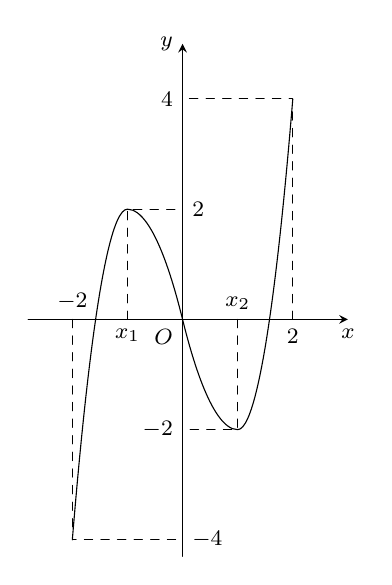
\begin{tikzpicture}[scale=0.7, font=\footnotesize, line join=round, line cap=round,>=stealth]
\def\a{1} \def\b{0} \def\c{-3} \def\d{0}
\def\xmin{-2.8} \def\xmax{3}
\def\ymin{-4.3} \def\ymax{5}
\draw[->] (\xmin,0)--(\xmax,0) node [below]{$x$};
\draw[->] (0,\ymin)--(0,\ymax) node [left]{$y$};
\node at (0,0) [below left]{$O$};
\clip (\xmin+0.1,\ymin+0.1) rectangle (\xmax-0.1,\ymax-0.1);
\draw (-2,-4) parabola bend (-1,2) (0,0)
parabola bend (1,-2) (2,4);
\draw[dashed] (-2,0)node[above]{$-2$}--(-2,-4)--(0,-4)node[right]{$-4$}
(2,0)node[below]{$2$}--(2,4)--(0,4)node[left]{$4$}
(-1,0)node[below]{$x_1$}--(-1,2)--(0,2)node[right]{$2$}
(1,0)node[above]{$x_2$}--(1,-2)--(0,-2)node[left]{$-2$}
;
\end{tikzpicture}
}
\loigiai{
Ta có số nghiệm của phương trình $|f(x)|=1$ là số giao điểm của đồ thị hàm số $y=|f(x)|$ với đường thẳng $y=1$.
\begin{center}
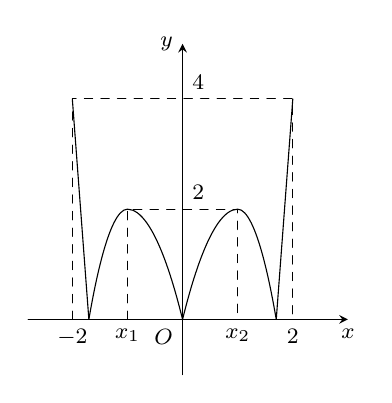
\begin{tikzpicture}[scale=0.7, font=\footnotesize, line join=round, line cap=round,>=stealth]
\def\a{1} \def\b{0} \def\c{-3} \def\d{0}
\def\xmin{-2.8} \def\xmax{3}
\def\ymin{-1} \def\ymax{5}
\draw[->] (\xmin,0)--(\xmax,0) node [below]{$x$};
\draw[->] (0,\ymin)--(0,\ymax) node [left]{$y$};
\node at (0,0) [below left]{$O$};
\clip (\xmin+0.1,\ymin+0.1) rectangle (\xmax-0.1,\ymax-0.1);
\draw (-2,4)--(-1.7,0) parabola bend (-1,2) (0,0)
parabola bend (1,2) (1.7,0)--(2,4);
\draw[dashed] (-2,0)node[below]{$-2$}--(-2,4)--(0,4)node[above right]{$4$}
--(2,4)--(2,0)node[below]{$2$}
(-1,0)node[below]{$x_1$}--(-1,2)--(0,2)node[above right]{$2$}
--(1,2)--(1,0)node[below]{$x_2$}
;
\end{tikzpicture}
\end{center}
Từ hình vẽ ta thấy đường thẳng $y=1$ cắt đồ thị hàm số $y=|f(x)|$ tại $6$ điểm.\\
Vậy số nghiệm của phương trình $|f(x)|=1$ là $6$.}
\end{ex}

%%% CÂU 21
\begin{ex}%[2D1Y5-4]
[Mã 102 - 2020 Lần 2] Cho hàm số bậc bốn $y=f(x)$ có đồ thị là đường cong trong hình vẽ bên. Số nghiệm thực của phương trình $f(x)=-\dfrac{3}{2}$ là
\begin{center}
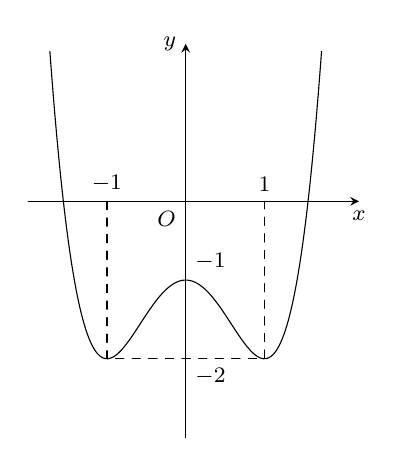
\begin{tikzpicture}[scale=1, font=\footnotesize, line join=round, line cap=round,>=stealth]
\def\a{1} \def\b{-2} \def\c{-1}
\def\xmin{-2} \def\xmax{2.2}
\def\ymin{-3} \def\ymax{2}
\draw[->] (\xmin,0)--(\xmax,0) node [below]{$x$};
\draw[->] (0,\ymin)--(0,\ymax) node [left]{$y$};
\node at (0,0) [below left]{$O$};
\clip (\xmin+0.1,\ymin+0.1) rectangle (\xmax-0.1,\ymax-0.1);
\draw[smooth,samples=300] plot(\x,{\a*(\x)^4+\b*(\x)^2+\c});
\draw[dashed] (-1,0)node[above]{$-1$}--(-1,-2)--(1,-2)--(1,0)node[above ]{$1$};
\draw (0,-1)node[above right]{$-1$} (0,-2)node[below right]{$-2$};
\end{tikzpicture}
\end{center}
\choice
{\True $4$}
{$1$}
{$3$}
{$2$}
\loigiai{
Từ đồ thị ta $f(x)=-\dfrac{3}{2}$ có $4$ nghiệm phân biệt.}
\end{ex}

%%% CÂU 22
\begin{ex}%[2D1Y5-4]
[Mã 103 - 2020 Lần 2] Cho hàm số bậc bốn $y=f(x)$ có đồ thị là đường cong trong hình bên. Số nghiệm thực của phương trình $f(x)=\dfrac{1}{2}$ là
\begin{center}
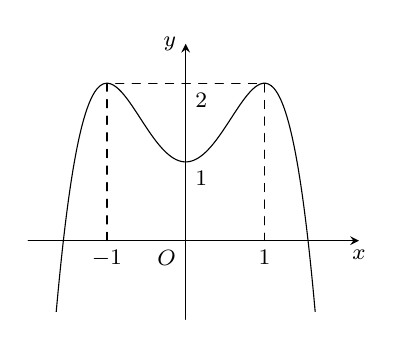
\begin{tikzpicture}[scale=1, font=\footnotesize, line join=round, line cap=round,>=stealth]
\def\a{-1} \def\b{2} \def\c{1}
\def\xmin{-2} \def\xmax{2.2}
\def\ymin{-1} \def\ymax{2.5}
\draw[->] (\xmin,0)--(\xmax,0) node [below]{$x$};
\draw[->] (0,\ymin)--(0,\ymax) node [left]{$y$};
\node at (0,0) [below left]{$O$};
\clip (\xmin+0.1,\ymin+0.1) rectangle (\xmax-0.1,\ymax-0.1);
\draw[smooth,samples=300] plot(\x,{\a*(\x)^4+\b*(\x)^2+\c});
\draw[dashed] (-1,0)node[below]{$-1$}--(-1,2)--(1,2)--(1,0)node[below]{$1$};
\draw (0,1)node[below right]{$1$} (0,2)node[below right]{$2$};
\end{tikzpicture}
\end{center}
\choice
{\True $2$}
{$4$}
{$1$}
{$3$}
\loigiai{
Số nghiệm thực của phương trình $f(x)=\dfrac{1}{2}$ chính là số giao điểm của đồ thị hàm số $f(x)$ với đường thẳng $y=\dfrac{1}{2}$.
\begin{center}
\begin{tikzpicture}[scale=1, font=\footnotesize, line join=round, line cap=round,>=stealth]
\def\a{-1} \def\b{2} \def\c{1}
\def\xmin{-2} \def\xmax{2.2}
\def\ymin{-1} \def\ymax{2.5}
\draw[->] (\xmin,0)--(\xmax,0) node [below]{$x$};
\draw[->] (0,\ymin)--(0,\ymax) node [left]{$y$};
\node at (0,0) [below left]{$O$};
\clip (\xmin+0.1,\ymin+0.1) rectangle (\xmax-0.1,\ymax-0.1);
\draw[smooth,samples=300] plot(\x,{\a*(\x)^4+\b*(\x)^2+\c});
\draw[dashed] (-1,0)node[below]{$-1$}--(-1,2)--(1,2)--(1,0)node[below]{$1$};
\draw (0,1)node[below right]{$1$} (0,2)node[below right]{$2$};
\draw (-2,0.5)--(2,0.5) (1.7,0.5)node[above]{$y=\dfrac{1}{2}$};
\end{tikzpicture}
\end{center}
Dựa vào hình trên ta thấy đồ thị hàm số $f(x)$ với đường thẳng $y=\dfrac{1}{2}$ có $2$ giao điểm.\\
Vậy phương trình $f(x)=\dfrac{1}{2}$ có hai nghiệm.}
\end{ex}

%%% CÂU 23
\begin{ex}[Mã 101 – 2020 Lần 2] %[2D1Y5-4]
Cho hàm số bậc bốn $y=f(x)$ có đồ thị là đường cong trong hình bên.
\begin{center}
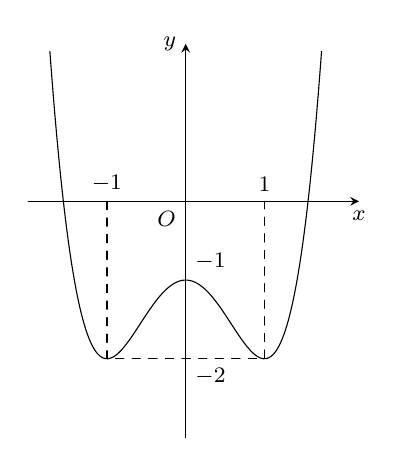
\begin{tikzpicture}[scale=1, font=\footnotesize, line join=round, line cap=round,>=stealth]
\def\a{1} \def\b{-2} \def\c{-1}
\def\xmin{-2} \def\xmax{2.2}
\def\ymin{-3} \def\ymax{2}
\draw[->] (\xmin,0)--(\xmax,0) node [below]{$x$};
\draw[->] (0,\ymin)--(0,\ymax) node [left]{$y$};
\node at (0,0) [below left]{$O$};
\clip (\xmin+0.1,\ymin+0.1) rectangle (\xmax-0.1,\ymax-0.1);
\draw[smooth,samples=300] plot(\x,{\a*(\x)^4+\b*(\x)^2+\c});
\draw[dashed] (-1,0)node[above]{$-1$}--(-1,-2)--(1,-2)--(1,0)node[above ]{$1$};
\draw (0,-1)node[above right]{$-1$} (0,-2)node[below right]{$-2$};
\end{tikzpicture}
\end{center}
Số nghiệm của phương trình $f(x)=-\dfrac{1}{2}$ là
\choice
{$3$}
{$4$}
{\True $2$}
{$x=1$}
\loigiai{
Số nghiệm của phương trình $f(x)=-\dfrac{1}{2}$ bằng số giao điểm của đồ thị hàm số $y=f(x)$ và đường thẳng $y=-\dfrac{1}{2}$.\\
Dựa vào đồ thị ta thấy: đồ thị hàm số $y=f(x)$ và đường thẳng $y=-\dfrac{1}{2}$ cắt nhau tại $2$ điểm.\\
Nên phương trình $f(x)=-\dfrac{1}{2}$ có 2 nghiệm.}
\end{ex}

%%% CÂU 24
\begin{ex}%[2D1Y5-4]
[Mã 104 - 2020 Lần 2] Cho hàm số $y=f(x)$ có đồ thị là đường cong trong hình bên. Số nghiệm thực của phương trình $f(x)=\dfrac{1}{2}$ là
\begin{center}
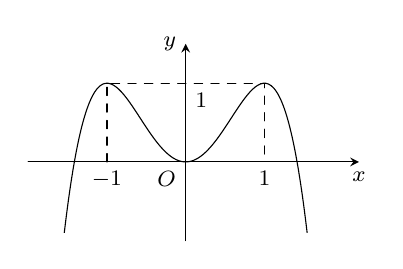
\begin{tikzpicture}[scale=1, font=\footnotesize, line join=round, line cap=round,>=stealth]
\def\a{-1} \def\b{2} \def\c{0}
\def\xmin{-2} \def\xmax{2.2}
\def\ymin{-1} \def\ymax{1.5}
\draw[->] (\xmin,0)--(\xmax,0) node [below]{$x$};
\draw[->] (0,\ymin)--(0,\ymax) node [left]{$y$};
\node at (0,0) [below left]{$O$};
\clip (\xmin+0.1,\ymin+0.1) rectangle (\xmax-0.1,\ymax-0.1);
\draw[smooth,samples=300] plot(\x,{\a*(\x)^4+\b*(\x)^2+\c});
\draw[dashed] (-1,0)node[below]{$-1$}--(-1,1)--(1,1)--(1,0)node[below]{$1$};
\draw (0,1)node[below right]{$1$};
\end{tikzpicture}
\end{center}
\choice
{\True $4$}
{$2$}
{$1$}
{$3$}
\loigiai{
\begin{center}
\begin{tikzpicture}[scale=1, font=\footnotesize, line join=round, line cap=round,>=stealth]
\def\a{-1} \def\b{2} \def\c{0}
\def\xmin{-2} \def\xmax{2.2}
\def\ymin{-1} \def\ymax{1.5}
\draw[->] (\xmin,0)--(\xmax,0) node [below]{$x$};
\draw[->] (0,\ymin)--(0,\ymax) node [left]{$y$};
\node at (0,0) [below left]{$O$};
\clip (\xmin+0.1,\ymin+0.1) rectangle (\xmax-0.1,\ymax-0.1);
\draw[smooth,samples=300] plot(\x,{\a*(\x)^4+\b*(\x)^2+\c});
\draw[dashed] (-1,0)node[below]{$-1$}--(-1,1)--(1,1)--(1,0)node[below]{$1$};
\draw (0,1)node[below right]{$1$} (-2,0.5)--(2,0.5) (1.2,0.5)node[above right]{$y=\dfrac{1}{2}$};
\end{tikzpicture}
\end{center}
Số nghiệm thực của phương trình $f(x)=\dfrac{1}{2}$ bằng số giao điểm của đường thẳng $y=\dfrac{1}{2}$ và có đồ thị hàm số $y=f(x)$.\\
Ta thấy đường thẳng $y=\dfrac{1}{2}$ cắt đồ thị hàm số tại $4$ điểm nên phương trình $f(x)=\dfrac{1}{2}$ có $4$ nghiệm.
}
\end{ex}

%%% CÂU 25
\begin{ex}%[2D1Y5-4]
[Mã 101-2022] Cho hàm số $f(x)=ax^4+bx^2+c$ có đồ thị là đường cong trong hình bên
\begin{center}
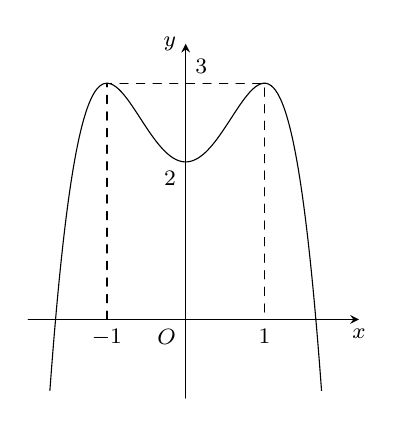
\begin{tikzpicture}[scale=1, font=\footnotesize, line join=round, line cap=round,>=stealth]
\def\a{-1} \def\b{2} \def\c{2}
\def\xmin{-2} \def\xmax{2.2}
\def\ymin{-1} \def\ymax{3.5}
\draw[->] (\xmin,0)--(\xmax,0) node [below]{$x$};
\draw[->] (0,\ymin)--(0,\ymax) node [left]{$y$};
\node at (0,0) [below left]{$O$};
\clip (\xmin+0.1,\ymin+0.1) rectangle (\xmax-0.1,\ymax-0.1);
\draw[smooth,samples=300] plot(\x,{\a*(\x)^4+\b*(\x)^2+\c});
\draw[dashed] (-1,0)node[below]{$-1$}--(-1,3)--(1,3)--(1,0)node[below]{$1$};
\draw (0,3)node[above right]{$3$} (0,2)node[below left]{$2$};
\end{tikzpicture}
\end{center}
Số nghiệm thực của phương trình $f(x)=1$.
\choice
{$1$}
{\True $2$}
{$4$}
{$3$}
\loigiai{
Đường thẳng $(d)$ có phương trình $y=1$ cắt đồ thị hàm số $y=f(x)$ tại $2$ điểm phân biệt.
\begin{center}
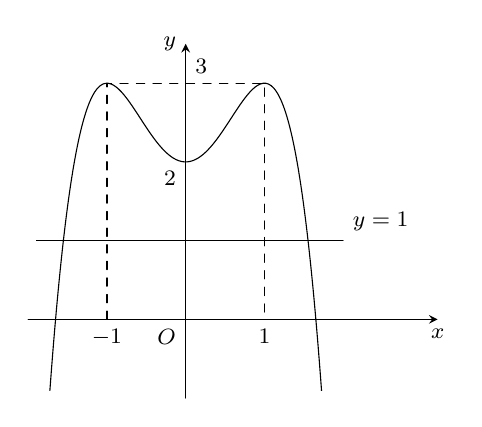
\begin{tikzpicture}[scale=1, font=\footnotesize, line join=round, line cap=round,>=stealth]
\def\a{-1} \def\b{2} \def\c{2}
\def\xmin{-2} \def\xmax{3.2}
\def\ymin{-1} \def\ymax{3.5}
\draw[->] (\xmin,0)--(\xmax,0) node [below]{$x$};
\draw[->] (0,\ymin)--(0,\ymax) node [left]{$y$};
\node at (0,0) [below left]{$O$};
\clip (\xmin+0.1,\ymin+0.1) rectangle (\xmax-0.1,\ymax-0.1);
\draw[smooth,samples=300] plot(\x,{\a*(\x)^4+\b*(\x)^2+\c});
\draw[dashed] (-1,0)node[below]{$-1$}--(-1,3)--(1,3)--(1,0)node[below]{$1$};
\draw (0,3)node[above right]{$3$} (0,2)node[below left]{$2$}
(-2,1)--(2,1)node[above right]{$y=1$};
\end{tikzpicture}
\end{center}
Suy ra phương trình $f(x)=1$ có $2$ nghiệm thực phân biệt.
}
\end{ex}

%%% CÂU 26
\begin{ex}%[2D1Y5-4]
[Mã 102 - 2022] Cho hàm số $f(x)=ax^4+bx^2+c$ có đồ thị là đường cong trong hình vẽ sau
\begin{center}
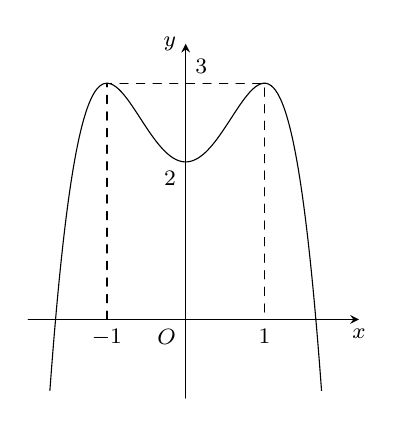
\begin{tikzpicture}[scale=1, font=\footnotesize, line join=round, line cap=round,>=stealth]
\def\a{-1} \def\b{2} \def\c{2}
\def\xmin{-2} \def\xmax{2.2}
\def\ymin{-1} \def\ymax{3.5}
\draw[->] (\xmin,0)--(\xmax,0) node [below]{$x$};
\draw[->] (0,\ymin)--(0,\ymax) node [left]{$y$};
\node at (0,0) [below left]{$O$};
\clip (\xmin+0.1,\ymin+0.1) rectangle (\xmax-0.1,\ymax-0.1);
\draw[smooth,samples=300] plot(\x,{\a*(\x)^4+\b*(\x)^2+\c});
\draw[dashed] (-1,0)node[below]{$-1$}--(-1,3)--(1,3)--(1,0)node[below]{$1$};
\draw (0,3)node[above right]{$3$} (0,2)node[below left]{$2$};
\end{tikzpicture}
\end{center}
Số nghiệm thực của phương trình $f(x)=1$ là
\choice
{$4$}
{$3$}
{\True $2$}
{$1$}
\loigiai{
\begin{center}
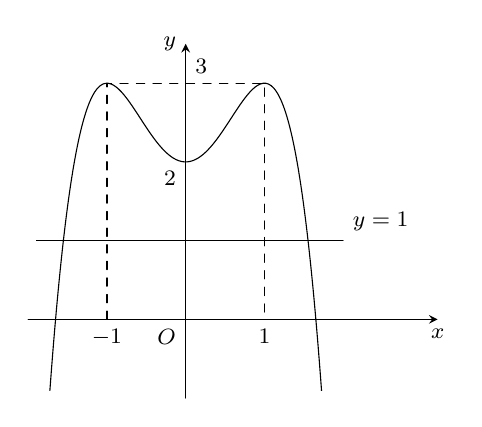
\begin{tikzpicture}[scale=1, font=\footnotesize, line join=round, line cap=round,>=stealth]
\def\a{-1} \def\b{2} \def\c{2}
\def\xmin{-2} \def\xmax{3.2}
\def\ymin{-1} \def\ymax{3.5}
\draw[->] (\xmin,0)--(\xmax,0) node [below]{$x$};
\draw[->] (0,\ymin)--(0,\ymax) node [left]{$y$};
\node at (0,0) [below left]{$O$};
\clip (\xmin+0.1,\ymin+0.1) rectangle (\xmax-0.1,\ymax-0.1);
\draw[smooth,samples=300] plot(\x,{\a*(\x)^4+\b*(\x)^2+\c});
\draw[dashed] (-1,0)node[below]{$-1$}--(-1,3)--(1,3)--(1,0)node[below]{$1$};
\draw (0,3)node[above right]{$3$} (0,2)node[below left]{$2$}
(-2,1)--(2,1)node[above right]{$y=1$};
\end{tikzpicture}
\end{center}
Số nghiệm thực của phương trình $f(x)=1$ bằng với số giao điểm của đường thẳng $(d)\colon y=1$ và đồ thị $(C)$ của hàm số $y=f(x)$. Dựa vào hình vẽ, ta thấy $(d)$ và $(C)$ cắt nhau tại hai điểm phân biệt nên phương trình đã cho có hai nghiệm thực phân biệt}
\end{ex}

%%% CÂU 27
\begin{ex}%[2D1Y5-4]
[Mã 103-2022] Cho hàm số $y=f(x)$ có bảng biến thiên như sau
\begin{center}

\begin{tikzpicture}
\tkzTabInit[nocadre=true,lgt=1.2,espcl=2.5,deltacl=0.6]
{$x$ /0.6, $y'$ /0.6, $y$ /2.5}
{$-\infty$,$0$,$2$,$+\infty$}
\tkzTabLine{,-,$0$,+,$0$,-,}
\tkzTabVar{+/$+\infty$,-/$-1$,+/$3$,-/$-\infty$}
\end{tikzpicture}
\end{center}
Số giao điểm của đồ thị hàm số đã cho và đường thẳng $y=1$ là
\choice
{$1$}
{$0$}
{$2$}
{\True $3$}
\loigiai{
\begin{center}
\begin{tikzpicture}
\tkzTabInit[nocadre=true,lgt=1.2,espcl=2.5,deltacl=0.6]
{$x$ /0.6, $y'$ /0.6, $y$ /2.5}
{$-\infty$,$0$,$2$,$+\infty$}
\tkzTabLine{,-,$0$,+,$0$,-,}
\tkzTabVar{+/$+\infty$,-/$-1$,+/$3$,-/$-\infty$}
\draw (1.4,-2)--(9,-2)node[above]{$y=1$};
\end{tikzpicture}
\end{center}
Dựa vào bảng biến thiên ta thấy đường thẳng $y=1$ cắt đồ thị hàm số tại 3 điểm}
\end{ex}

%%% CÂU 28
\begin{ex}%[2D1B5-4]
[Mã 103 - 2022] Cho hàm số $f(x)=a x^4+b x^2+c$ có đồ thị là đường cong trong hình bên. Có bao nhiêu giá trị nguyên thuộc đoạn $[-2; 5]$ của tham số $m$ để phương trình $f(x)=m$ có đúng $2$ nghiệm thực phân biệt?
\begin{center}
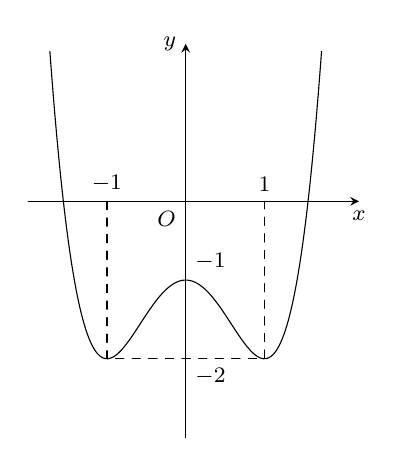
\begin{tikzpicture}[scale=1, font=\footnotesize, line join=round, line cap=round,>=stealth]
\def\a{1} \def\b{-2} \def\c{-1}
\def\xmin{-2} \def\xmax{2.2}
\def\ymin{-3} \def\ymax{2}
\draw[->] (\xmin,0)--(\xmax,0) node [below]{$x$};
\draw[->] (0,\ymin)--(0,\ymax) node [left]{$y$};
\node at (0,0) [below left]{$O$};
\clip (\xmin+0.1,\ymin+0.1) rectangle (\xmax-0.1,\ymax-0.1);
\draw[smooth,samples=300] plot(\x,{\a*(\x)^4+\b*(\x)^2+\c});
\draw[dashed] (-1,0)node[above]{$-1$}--(-1,-2)--(1,-2)--(1,0)node[above ]{$1$};
\draw (0,-1)node[above right]{$-1$} (0,-2)node[below right]{$-2$};
\end{tikzpicture}
\end{center}
\choice
{$1$}
{$6$}
{\True $7$}
{$5$}
\loigiai{
Dựa vào đồ thị ta thấy phương trình $f(x)=m$ có đúng hai nghiệm thực phân biệt khi $m=-2$.\\
Hoặc $m>-1$. Vậy $m\in\{-2; 0; 1; 2; 3; 4; 5\}$. Vậy có $7$ giá trị $m$ thĩa mãn}
\end{ex}

%%% CÂU 29
\begin{ex}%[2D1Y5-4]
[Mã 104-2022] Cho hàm số $y=f(x)$ có bảng biến thiên như sau
\begin{center}

\begin{tikzpicture}
\tkzTabInit[nocadre=true,lgt=1.2,espcl=2.5,deltacl=0.6]
{$x$ /0.6, $y'$ /0.6, $y$ /2.5}
{$-\infty$,$0$,$2$,$+\infty$}
\tkzTabLine{,-,$0$,+,$0$,-,}
\tkzTabVar{+/$+\infty$,-/$-1$,+/$3$,-/$-\infty$}
\end{tikzpicture}
\end{center}
Số giao điểm của đồ thị hàm số đã cho và đường thẳng $y=1$ là
\choice
{$2$}
{$1$}
{\True $3$}
{$0$}
\loigiai{
Ta vẽ đường thẳng $y=1$.
\begin{center}
\begin{tikzpicture}
\tkzTabInit[nocadre=true,lgt=1.2,espcl=2.5,deltacl=0.6]
{$x$ /0.6, $y'$ /0.6, $y$ /2.5}
{$-\infty$,$0$,$2$,$+\infty$}
\tkzTabLine{,-,$0$,+,$0$,-,}
\tkzTabVar{+/$+\infty$,-/$-1$,+/$3$,-/$-\infty$}
\draw (1.4,-2)--(9,-2)node[above]{$y=1$};
\end{tikzpicture}
\end{center}
Đường thẳng $y=1$ cắt đồ thị hàm số tại $3$ giao điểm.}
\end{ex}

%%% CÂU 30
\begin{ex}%[2D1B5-4]
[Mã 104-2022] Cho hàm số $f(x)=ax^4+bx^2+c$ có đồ thị là đường cong trong hình bên dưới.
\begin{center}
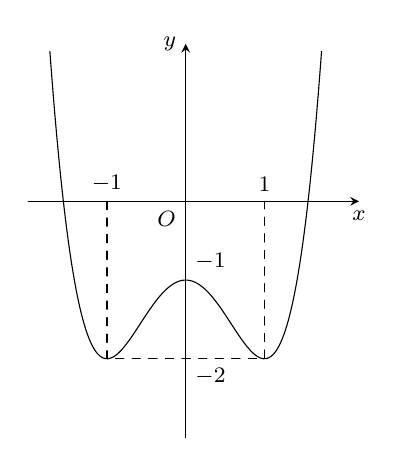
\begin{tikzpicture}[scale=1, font=\footnotesize, line join=round, line cap=round,>=stealth]
\def\a{1} \def\b{-2} \def\c{-1}
\def\xmin{-2} \def\xmax{2.2}
\def\ymin{-3} \def\ymax{2}
\draw[->] (\xmin,0)--(\xmax,0) node [below]{$x$};
\draw[->] (0,\ymin)--(0,\ymax) node [left]{$y$};
\node at (0,0) [below left]{$O$};
\clip (\xmin+0.1,\ymin+0.1) rectangle (\xmax-0.1,\ymax-0.1);
\draw[smooth,samples=300] plot(\x,{\a*(\x)^4+\b*(\x)^2+\c});
\draw[dashed] (-1,0)node[above]{$-1$}--(-1,-2)--(1,-2)--(1,0)node[above ]{$1$};
\draw (0,-1)node[above right]{$-1$} (0,-2)node[below right]{$-2$};
\end{tikzpicture}
\end{center}
Có bao nhiêu giá trị nguyên thuộc đoạn $[-2; 5]$ của tham số $m$ để phương trình $f(x)=m$ có đúng $2$ nghiệm thực phân biệt?
\choice
{\True $7$}
{$6$}
{$5$}
{$1$}
\loigiai{
Ta có yêu cầu bài toán tương đương với $\hoac{&m=-2\\& m>-1.}$ \\
Do $m\in[-2; 5]$ và $m$ nguyên nên có $7$ giá trị $m$ cần tìm là $-2,0,1,2,3,4,5$.}
\end{ex}
\begin{dang}{Bài toán tương giao đồ thị thông qua hàm số cho trước}
\end{dang}
%%% CÂU 31
\begin{ex}%[2D1Y5-4]
	[Đề Minh Họa 2021] Đồ thị của hàm số $y=x^3-3x+2$ cắt trục tung tại điểm có tung độ bằng
	\choice
	{$0$}
	{$1$}
	{\True $2$}
	{$-2$}
	\loigiai{
		Gọi $M(x_0; y_0)$ là giao điểm của đồ thị hàm số với trục tung. Ta có $x_0=0\Rightarrow y_0=2$}
\end{ex}

%%% CÂU 32
\begin{ex}%[2D1Y5-4]
	[Mã 101 - 2021 Lần 1] Đồ thị hàm số $y=-x^4+4 x^2-3$ cắt trục tung tại điểm có tung độ bằng
	\choice
	{$0$}
	{$3$}
	{$1$}
	{\True $-3$}
	\loigiai{
		Đồ thị hàm số $y=-x^4+4 x^2-3$ sẽ cắt trục tung tại điểm có hoành độ $x=0$.\\
		Từ đó ta được $y=-3$}
\end{ex}

%%% CÂU 33
\begin{ex}%[2D1Y5-4]
	[Mã 103 - 2021 Lần 1] Đồ thị hàm số $y=-x^3+2x^2-1$ cắt trục tung tại điểm có tung độ bằng
	\choice
	{$3$}
	{$1$}
	{\True $-1$}
	{$0$}
	\loigiai{
		Từ hàm số: $y=-x^3+2x^2-1$, cho $x=0\Rightarrow y=-1$.\\
		Vậy đồ thị hàm số $y=-x^3+2 x^2-1$ cắt trục tung tại điểm có tung độ bằng $-1$.}
\end{ex}

%%% CÂU 34
\begin{ex}%[2D1Y5-4]
	[Mã 102 - 2021 Lần 1] Đồ thị của hàm số $y=-x^4-2 x^2+3$ cắt trục tung tại điểm có tung độ bằng
	\choice
	{$1$}
	{$0$}
	{$2$}
	{\True $3$}
	\loigiai{
		Giả sử $y=-x^4-2 x^2+3. \quad(C)$\\
		Gọi $(C)\cap Oy=M(x_0; y_0)\Rightarrow x_0=0\Rightarrow y_0=3$.\\
		Vậy đồ thị của hàm số $y=-x^4-2 x^2+3$ cắt trục tung tại điểm có tung độ bằng 3}
\end{ex}

%%% CÂU 35
\begin{ex}%[2D1Y5-4]
	[Mã 104 - 2021 Lần 1] Đồ thị của hàm số $y=-2 x^3+3 x^2-5$ cắt trục tung tại điểm có tung độ bằng
	\choice
	{\True $-5$}
	{$0$}
	{$-1$}
	{$2$}
	\loigiai{
		Gọi $M(x_0; y_0)$ là giao điểm của đồ thị hàm số $y=-2 x^3+3 x^2-5$ và trục tung, ta có: $x_0=0\Rightarrow y_0=-5$}
\end{ex}

%%% CÂU 36
\begin{ex}%[2D1B5-4]
	[Đề Tham Khảo 2020 Lần 2] Số giao điểm của đồ thị hàm số $y=x^3-3x+1$ và trục hoành là
	\choice
	{\True $3$}
	{$0$}
	{$2$}
	{$1$}
	\loigiai{
		Tập xác định $\mathbb{R}$.\\
		Ta có: $y'=3x^2-3=3\left(x^2-1\right);y'=0\Leftrightarrow x=\pm 1$.\\
		Bảng biến thiên
		\begin{center}
			
\begin{tikzpicture}
				\tkzTabInit[nocadre=true,lgt=1.2,espcl=2.5,deltacl=0.6]
				{$x$ /0.6, $y'$ /0.6, $y$ /2.5}
				{$-\infty$,$-1$,$1$,$+\infty$}
				\tkzTabLine{,+,$0$,-,$0$,+,}
				\tkzTabVar{-/$-\infty$,+/$3$,-/$-1$,+/$+\infty$}
			\end{tikzpicture}
		\end{center}
		Từ bảng biến thiên ta thấy đồ thị hàm số cắt trục hoành tại $3$ điểm phân biệt.}
\end{ex}

%%% CÂU 37
\begin{ex}%[2D1B5-4]
	[Mã 101 - 2020 Lần 1] Số giao điểm của đồ thị hàm số $y=x^3+3x^2$ và đồ thị hàm số $y=3x^2+3x$ là
	\choice
	{\True $3$}
	{$1$}
	{$2$}
	{$0$}
	\loigiai{
		Phương trình hoành độ giao điểm của hai đồ thị đã cho là\\
		$x^3+3x^2=3x^2+3x\Leftrightarrow x^3-3x=0\Leftrightarrow x\left(x^2-3\right)=0\Leftrightarrow\hoac{&x=0\\&x=\sqrt{3}\\&x=-\sqrt{3}.}$ \\
		Hai đồ thị đã cho cắt nhau tại $3$ điểm.}
\end{ex}

%%% CÂU 38
\begin{ex}%[2D1B5-4]
	[Mã 102 - 2020 Lần 1] Số giao điểm của đồ thị hàm số $y=x^3-x^2$ và đồ thị hàm số $y=-x^2+5x$ là
	\choice
	{$2$}
	{\True $3$}
	{$1$}
	{$0$}
	\loigiai{
		Số giao điểm của đồ thị hàm số $y=x^3-x^2$ và đồ thị hàm số $y=-x^2+5x$ chính là số nghiệm thực của phương trình $x^3-x^2=-x^2+5x\Leftrightarrow x^3-5x=0\Leftrightarrow\hoac{&x=0\\&x=\pm\sqrt{5}}$.}
\end{ex}

%%% CÂU 39
\begin{ex}%[2D1B5-4]
	[Mã 103 - 2020 Lần 1] Số giao điểm của đồ thị hàm số $y=x^3+x^2$ và đồ thị hàm số $y=x^2+5x$.
	\choice
	{\True $3$}
	{$0$}
	{$1$}
	{$2$}
	\loigiai{
		Phương trình hoành độ giao điểm: $x^3+x^2=x^2+5x\Leftrightarrow x^3-5x=0\Leftrightarrow\hoac{&x=0\\&x=\pm\sqrt{5}}$. \\
		Vậy số giao điểm của hai đồ thị là $3$.}
\end{ex}

%%% CÂU 40
\begin{ex}%[2D1B5-4]
	[Mã 104 - 2020 Lần 1] Số giao điểm của đồ thị hàm số $y=-x^2+3x$ và đồ thị hàm số $y=x^3-x^2$ là
	\choice
	{$1$}
	{$0$}
	{$2$}
	{\True $3$}
	\loigiai{
		Phương trình hoành độ giao điểm của hai đồ thị là $x^3-x^2=-x^2+3x\Leftrightarrow x^3-3x=0\Leftrightarrow\hoac{&x=0\\&x=\pm\sqrt{3}}$.}
\end{ex}

%%% CÂU 41
\begin{ex}%[2D1Y5-4]
	[Mã 102 - 2020 Lần 2] Số giao điểm của đồ thị hàm số $y=-x^3+7x$ với trục hoành là
	\choice
	{$0$}
	{\True $3$}
	{$2$}
	{$1$}
	\loigiai{
		Phương trình hoành độ giao điểm của đồ thị và trục hoành là \\
		$-x^3+7x=0\Leftrightarrow x\left(x^2-7\right)=0\Leftrightarrow\hoac{&x=0\\&x=\pm\sqrt{7}.}$ \\
		Số giao điểm của đồ thị hàm số $y=-x^3+7x$ với trục hoành bằng $3$.}
\end{ex}

%%% CÂU 42
\begin{ex}%[2D1Y5-4]
	[Mã 103 - 2020 Lần 2] Số giao điểm của đồ thị hàm số $y=-x^3+3x$ với trục hoành là
	\choice
	{$2$}
	{$0$}
	{\True $3$}
	{$1$}
	\loigiai{
		Xét phương trình hoành dộ giao điểm $-x^3+3x=0\Leftrightarrow x(-x^2+3)=0\Leftrightarrow\hoac{&x=0\\&x=\pm\sqrt{3}}$. \\
		Vậy có 3 giao điểm.}
\end{ex}

%%% CÂU 43
\begin{ex}%[2D1Y5-4]
	[Mã 101 – 2020 Lần 2] Số giao điểm của đồ thị hàm số $y=-x^3+6x$ với trục hoành là
	\choice
	{$2$}
	{\True $3$}
	{$1$}
	{$0$}
	\loigiai{
		Ta có hoành độ giao điểm của đồ thị hàm số $y=-x^3+6x$ với trục hoành là nghiệm của phương trình\\
		$-x^3+6x=0\Leftrightarrow-x\left(x^2-6\right)=0\Leftrightarrow\hoac{&x=0\\&x=\pm\sqrt{6}.}$ \\
		Phương trình trên có ba nghiệm phân biệt, do đó đồ thị hàm số $y=-x^3+6x$ cắt trục hoành tại ba điểm phân biệt.}
\end{ex}

%%% CÂU 44
\begin{ex}%[2D1Y5-4]
	[Mã 104 - 2020 Lần 2] Số giao điểm của đồ thị hàm số $y=-x^3+5x$ với trục hoành là
	\choice
	{\True $3$}
	{$2$}
	{$0$}
	{$1$}
	\loigiai{
		Ta có $-x^3+5x=0\Leftrightarrow\hoac{&x=\sqrt{5}\\&x=-\sqrt{5}\\&x=0}$. \\
		Vậy số giao điểm của đồ thị hàm số $y=-x^3+5x$ với trục hoành là $3$.}
\end{ex}

%%% CÂU 45
\begin{ex}%[2D1Y5-4]
	[Mã 105 2017] Cho hàm số $y=(x-2)\left(x^2+1\right)$ có đồ thị $(C)$. Mệnh đề nào dưới đây đúng?
	\choice
	{\True $(C)$ cắt trục hoành tại một điểm}
	{$(C)$ cắt trục hoành tại ba điểm}
	{$(C)$ cắt trục hoành tại hai điểm}
	{$(C)$ không cắt trục hoành}
	\loigiai{
		Dễ thấy phương trình $(x-2)\left(x^2+1\right)=0$ có 1 nghiệm $x=2\Rightarrow (C)$ cắt trục hoành tại một điểm.}
\end{ex}

%%% CÂU 46
\begin{ex}%[2D1B5-4]
	[Đề Minh Họa 2017] Biết rằng đường thẳng $y=-2x+2$ cắt đồ thị hàm số $y=x^3+x+2$ tại điểm duy nhất; kí hiệu $(x_0;y_0)$ là tọa độ của điểm đó. Tìm $y_0$.
	\choice
	{$y_0=4$}
	{$y_0=0$}
	{\True $y_0=2$}
	{$y_0=-1$}
	\loigiai{
		Xét phương trình hoành độ giao điểm: $-2x+2=x^3+x+2\Leftrightarrow x^3+3x=0\Leftrightarrow x=0$.\\
		Với $x_0=0\Rightarrow y_0=2$.}
\end{ex}

%%% CÂU 47
\begin{ex}%[2D1B5-4]
	[THPT - Yên Định Thanh Hóa 2019] Gọi $P$ là số giao điểm của hai đồ thị $y=x^3-x^2+1$ và $y=x^2+1$. Tìm $P$.
	\choice
	{$P=0$}
	{\True $P=2$}
	{$P=1$}
	{$P=3$}
	\loigiai{
		Xét phương trình hoành độ giao điểm của hai đồ thị $y=x^3-x^2+1$ và $y=x^2+1$:\\
		$x^3-x^2+1=x^2+1\Leftrightarrow x^3-2x^2=0\Leftrightarrow\hoac{&x=0\\&x=2.}$ \\
		Với $x=0\Rightarrow y=1$.\\
		Với $x=2\Rightarrow y=5$.\\
		Nên hai đồ thị trên có hai giao điểm là $(0;1)$ và $(2;5)$.\\
		Vậy $P=2$.}
\end{ex}

%%% CÂU 48
\begin{ex}%[2D1Y5-4]
	[Đề Tham Khảo 2017] Cho hàm số $y=x^3-3x$ có đồ thị $(C)$. Tìm số giao điểm của $(C)$ và trục hoành.
	\choice
	{$2$}
	{\True $3$}
	{$1$}
	{$0$}
	\loigiai{
		Xét phương trình hoành độ giao điểm của $(C)$ và trục hoành: $x^3-3x=0\Leftrightarrow\hoac{&x=0\\&x=\pm\sqrt{3}}$. \\
		Vậy số giao điểm của $(C)$ và trục hoành là 3.}
\end{ex}

%%% CÂU 49
\begin{ex}%[2D1B5-4]
	[THPT Yên Khánh - Ninh Bình 2019] Cho hàm số $y=x^4-3x^2$ có đồ thị $(C)$. Số giao điểm của đồ thị $(C)$ và đường thẳng $y=2$ là
	\choice
	{\True $2$}
	{$1$}
	{$0$}
	{$4$}
	\loigiai{
		Số giao điểm của đồ thị $(C)$ và đường thẳng $y=2$ là số nghiệm của phương trình sau:\\
		$x^4-3x^2=2\Leftrightarrow x^4-3x^2-2=0\Leftrightarrow\hoac{&x^2=\dfrac{3+\sqrt{17}}{2}\\&x^2=\dfrac{3-\sqrt{17}}{2}<0}\Leftrightarrow x=\pm\sqrt{\dfrac{3+\sqrt{17}}{2}.}$ \\
		Phương trình hoành độ giao điểm có $2$ nghiệm nên số giao điểm của đồ thị $(C)$ và đường thẳng là $2$.}
\end{ex}

%%% CÂU 50
\begin{ex}%[2D1B5-4]
	[Chuyên Trần Phú Hải Phòng 2019] Biết rằng đường thẳng $y=4x+5$ cắt đồ thị hàm số $y=x^3+2x+1$ tại điểm duy nhất; kí hiệu $\left(x_0;y_0\right)$ là tọa độ của điểm đó. Tìm $y_0$.
	\choice
	{$y_0=10$}
	{\True $y_0=13$}
	{$y_0=11$}
	{$y_0=12$}
	\loigiai{
		Phương trình hoành độ giao điểm là $x^3+2x+1=4x+5\Leftrightarrow x^3-2x-4=0\Leftrightarrow x=2$.\\
		Với $x=2\Rightarrow y=13$. Vậy $y_0=13$.}
\end{ex}

%%% CÂU 51
\begin{ex}%[2D1Y5-4]
	[THPT Yên Phong 1 Bắc Ninh 2019] Đồ thị của hàm số $y=-x^4-3x^2+1$ cắt trục tung tại điểm có tung độ bao nhiêu
	\choice
	{$-3$}
	{$0$}
	{\True $1$}
	{$-1$}
	\loigiai{
		Trục tung có phương trình: $x=0$. Thay $x=0$ vào $y=-x^4-3x^2+1$ được: $y=1$.}
\end{ex}

%%% CÂU 52
\begin{ex}%[2D1B5-4]
	[THPT Việt Đức Hà Nội 2019] Số giao điểm của đường cong $y=x^3-2x^2+2x+1$ và đường thẳng $y=1-x$ là
	\choice
	{\True $1$}
	{$2$}
	{$3$}
	{$0$}
	\loigiai{
		Xét phương trình hoành độ giao điểm.\\
		$\begin{aligned}&x^3-2x^2+2x+1=1-x\\&\Leftrightarrow x^3-2x^2+3x=0\\&\Leftrightarrow x\left(x^2-2x+3\right)=0\Leftrightarrow x=0.\end{aligned}$}
\end{ex}

%%% CÂU 53
\begin{ex}%[2D1B5-4]
	Đồ thị hàm số $y=x^4-3x^2+1$ và đồ thị hàm số $y=-2x^2+7$ có bao nhiêu điểm chung?
	\choice
	{$0$}
	{$1$}
	{\True $2$}
	{$3$}
	\loigiai{
		Phương trình hoành độ giao điểm:\\
		$x^4-3x^2+1=-2x^2+7\Leftrightarrow x^4-x^2-6=0\Leftrightarrow\hoac{&x^2=3\\&x^2=-2}\Leftrightarrow x=\pm\sqrt{3.}$ \\
		Do pt có $2$ nghiệm nên đồ thị hai hàm số có $2$ điểm chung.}
\end{ex}

%%% CÂU 54
\begin{ex}%[2D1Y5-4]
	Cho hàm số $y=-2x^3+5x$ có đồ thị $(C)$ Tìm số giao điểm của $(C)$ và trục hoành.
	\choice
	{$2$}
	{\True $3$}
	{$1$}
	{$0$}
	\loigiai{
		Phương trình hoành độ giao điểm của $(C)$ và trục hoành là\\
		$-2x^3+5x=0\Leftrightarrow\hoac{&x=0\\&x=\pm\sqrt{\dfrac{5}{2}}}$ có $3$ giao điểm.\\
		Chú ý: Ở bài toán này hoàn toàn có thể giải trực tiếp bằng Casio với phương trình $-2x^3+5x=0$, nhưng chắc chắn thao tác bấm máy sẽ chậm hơn việc tính tay(thậm chí bài này không cần nháp khi mà kết quả đã hiện ra luôn khi ta đọc đề xong). Vì vậy, Casio là điều không cần thiết với câu hỏi này.}
\end{ex}

%%% CÂU 55
\begin{ex}%[2D1Y5-4]
	Cho hàm số $y=(x-3)\left(x^2+2\right)$ có đồ thị $(C)$. Mệnh đề nào dưới đây đúng?
	\choice
	{$(C)$ cắt trục hoành tại hai điểm}
	{\True $(C)$ cắt trục hoành tại một điểm}
	{$(C)$ không cắt trục hoành}
	{$(C)$ cắt trục hoành tại ba điểm}
	\loigiai{
		Phương trình hoành độ giao điểm của $(C)$ và trục hoành là\\
		$(x-3)\left(x^2+2\right)=0\Leftrightarrow\hoac{&x=3\\&x^2=-2}\Leftrightarrow x=3$ nghĩa là $(C)$ cắt trục hoành tại một điểm.}
\end{ex}

%%% CÂU 56
\begin{ex}%[2D1B5-4]
	Biết rằng đường thẳng $y=x+2$ cắt đồ thị hàm số $y=x^3-x^2+x+4$ tại điểm duy nhất, kí hiệu $(x_0;y_0)$ là tọa độ của điểm đó. Tìm $y_0$.
	\choice
	{\True $y_0=1$}
	{$y_0=3$}
	{$y_0=-2$}
	{$y_0=4$}
	\loigiai{
		Phương trình hoành độ giao điểm\\
		$x+2=x^3-x^2+x+4\Leftrightarrow x^3-x^2+2=0\Leftrightarrow x=-1\Rightarrow y_0=1$.}
\end{ex}

%%% CÂU 57
\begin{ex}%[2D1Y5-4]
	Đồ thị hàm số nào sau đây cắt trục tung tại điểm có tung độ âm?
	\choice
	{$y=\dfrac{x-1}{x-3}$}
	{$y=\dfrac{x+1}{x+4}$}
	{\True $y=\dfrac{x-1}{x+2}$}
	{$y=\dfrac{2x+1}{x+5}$}
	\loigiai{
		Trục tung có phương trình $x=0$, ta thay $x=0$ lần lượt vào các phương án thì chỉ có phương án C cho ta $y=-\dfrac{1}{2}<0$.}
\end{ex}

%%% CÂU 58
\begin{ex}%[2D1B5-4]
	Gọi $M,N$ là giao điểm của đường thẳng $y=x+1$ và đường cong $y=\dfrac{2x+4}{x-1}$. Khi đó hoành độ $x_I$ của trung điểm $I$ của đoạn $MN$ bằng bao nhiêu?
	\choice
	{$x_I=2$}
	{\True $x_I=1$}
	{$x_I=-5$}
	{$x_I=-\dfrac{5}{2}$}
	\loigiai{
		Điều kiện: $x\neq 1$.\\
		Phương trình hoành độ giao điểm $\dfrac{2x+4}{x-1}=x+1\Leftrightarrow x^2-2x-5=0\Leftrightarrow \hoac{& x_M=1+\sqrt{6}\\ & x_N=1-\sqrt{6}}$.\\
		Khi đó $x_I=\dfrac{x_M+x_N}{2}=1$.}
\end{ex}

%%% CÂU 59
\begin{ex}%[2D1B5-4]
	Cho hàm số $y=\dfrac{x+1}{x-3}$ có đồ thị $(C)$ và các đường thẳng $d_1\colon y=2x$, $d_2\colon y=2x-2$, $d_3\colon y=3x+3$, $d_4\colon y=-x+3$. Hỏi có bao nhiêu đường thẳng trong bốn đường thẳng $d_1$, $d_2$, $d_3$, $d_4$ đi qua giao điểm của $(C)$ và trục hoành.
	\choice
	{\True $1$}
	{$2$}
	{$3$}
	{$4$}
	\loigiai{
		Ta có $(C)$ cắt trục hoành $(y=0)$ tại điểm $M(-1;0)$.\\
		Trong các đường thẳng $d_1,d_2,d_3,d_4$ chỉ có $M\in d_3$, có nghĩa là có $1$ đường thẳng đi qua $M(-1;0)$.}
\end{ex}

%%% CÂU 60
\begin{ex}%[2D1K5-4]
	[THPT Quang Trung Đống Đa Hà Nội 2019] Tìm số giao điểm của đồ thị hàm số $y=\sqrt{x^4-4}+5$ và đường thẳng $y=x$.
	\choice
	{$3$}
	{\True $0$}
	{$2$}
	{$1$}
	\loigiai{
		\textbf{Cách 1:} Phương trình hoành độ giao điểm $\sqrt{x^4-4}+5=x\Leftrightarrow\sqrt{x^4-4}=x-5$\\
		$ \Leftrightarrow\heva{&x\geq 5\\&x^4-4=(x-5)^2} $ \\
		$ \Leftrightarrow\heva{&x\geq 5\\&x^4-x^2+10x-29=0 \quad(*).} $ \\
		Do $x\geq 5$ nên $x^4-x^2=x^2(x^2-1)>0$ và $10x-29>0$. Vì vậy $(*)$ vô nghiệm.\\
		Như vậy phương trình $\sqrt{x^4-4}+5=x$ vô nghiệm hay đồ thị hàm số $y=\sqrt{x^4-4}+5$ và đường thẳng $y=x$ không có giao điểm nào.\\
		\textbf{Cách 2.}
		Phương trình hoành độ giao điểm $\sqrt{x^4-4}+5=x$. Ta có điều kiện xác định $\hoac{&x\geq\sqrt{2}\\&x\leq-\sqrt{2}}$.\\
		Với điều kiện trên ta có $\sqrt{x^4-4}+5=x\Leftrightarrow\sqrt{x^4-4}+5-x=0$.\\
		Xét hàm số $h(x)=\sqrt{x^4-4}+5-x$.\\
		Ta có $h'(x)=\dfrac{2x^3}{\sqrt{x^4-4}}-1$; $h'(x)=0\Leftrightarrow 2x^3=\sqrt{x^4-4}$.\\
		Với $x\geq\sqrt{2}$ ta có $2x^3>\sqrt{x^4-4}$.\\
		Với $x\leq-\sqrt{2}$ ta có $2x^3<\sqrt{x^4-4}$.\\
		Ta có bảng biến thiên:
		\begin{center}
			
\begin{tikzpicture}
				\tkzTabInit[nocadre=true,lgt=1.2,espcl=2.5,deltacl=0.6]
				{$x$ /0.6,$h'(x)$ /0.6,$h(x)$ /2}
				{$-\infty$,$-\sqrt{2}$,$\sqrt{2}$,$+\infty$}
				\tkzTabLine{,-,d,,d,+,}
				\tkzTabVar{+/$+\infty$, -DH/$5+\sqrt{2}$,D-/$5-\sqrt{2}$,+/$+\infty$}
			\end{tikzpicture}
		\end{center}
		Số nghiệm của phương trình $\sqrt{x^4-4}+5=x$ là số giao điểm của đồ thị $y=h(x)=\sqrt{x^4-4}+5-x$ và trục hoành $y=0$. Dựa vào BBT ta thấy phương trình $\sqrt{x^4-4}+5=x$ vô nghiệm hay đồ thị hàm số $y=\sqrt{x^4-4}+5$ và đường thẳng $y=x$ không có giao điểm nào.
	}
\end{ex}
\Closesolutionfile{ans}
\indapan{10}{ans/CD6/Muc_5_6}